\documentclass{article}

\usepackage{spconf}
\usepackage{siunitx}
\usepackage{graphicx}
\usepackage{tabularx}
\usepackage[hidelinks]{hyperref}

\title{Raspberry Pi Driven Vision for Autonomous Mobility}
\name{Andrei Tumbar}
\address{Computer Engineering\\
Rochester Institute of Technology\\
at1777@rit.edu}

\begin{document}
\maketitle

\begin{abstract}
Classical computer vision has always been a challenge to implement on an embedded
systems because of the requirement of fast computational power and system memory.
This paper presents a possible solution to realtime computer vision aboard a
Raspberry Pi 3B for the purpose of driving an autonomous vehicle.
\end{abstract}

\section{Introduction}

Vision processing is a fairly well developed field that looks at processing images
to extract certain features. This can include features such as object edges, object
classification, or 3D mesh reconstruction with stereo correlation. One of the major
challenges of computer vision in robotics and other embedded systems arises from
vast computational requirements.

Many robots that operate from the input of a camera will use some form of computer
vision to drive their navigation logic. For example, the Perseverance rover uses
a combination of its 6 engineering cameras as well as an inertial measurement unit
for path planning and pose estimation \cite{b1}. One of the main challenges with
computer vision for robotics and other embedded system arises from the large computational
requirements of vision software. While algorithms are parallelizable making
graphics processing units (GPUs) highly attractive, power constraints of these robots
usually factors in to these robots.

There has been some work in the past done to implement vision on the Raspberry Pi. \cite{b3}
discusses a Raspberry Pi configuration that uses the Raspberry Pi camera module. OpenCV
is used to support much of the vision functionality. This project will use some of the
design decisions from \cite{b3} however will not used the Python OpenCV packages distributed
for the Raspberry Pi. Instead, a custom compiled, statically linked version of OpenCV is
built as well as a leaned down version Debian Linux operating system is used instead of
the one noted in \cite{b3}.

This paper introduces a vision and navigation system aboard a Raspberry Pi 3B. The official
Raspberry Pi Camera Module V2 is used for its impressive streaming features and hardware
noise reduction. The vision system is meant to drive a small battery powered car around
a track. The Raspberry Pi's low power requirements of \SI{3.7}{\watt} at maximum load
of all four internal cores makes it optimal for this application \cite{b2}. Unlike
robots mentioned previous in \cite{b1}, this vision system will only operate off of
a single camera. Depth estimation is performed using a calibrated camera pose and an
affine transform for adjusting camera perspective. This paper will discuss the
implementation details of the vision and navigation systems such as the software framework
used as well as the physical configuration of the car. 

\section{Background}

\subsection{TI Cup Car Hardware}

The purpose of this project is to drive a TI Cup Car. This car includes two direct current
(DC) motors used for throttle as well as a servo motor to control the steering arms.
All three motors are driven with a pulse-width modulation (PWM) signal. The DC motors
used for the rear wheels have a base frequency of \SI{10}{\kilo\hertz} while the steering
servo uses a frequency of \SI{50}{\hertz}. Due to the low current limitations of a software
drivable general purpose input/output (GPIO) pins, the DC motors cannot be switched directly
from the pin headers. A motor driver must be used to switch an external power source
controlled by a low drive GPIO. This motor drive H-bridge circuit able to
switch the high current requirement of the DC motors from the external battery under the
control of a \SI{3.3}{\volt} GPIO PWM signal.

One of the challenges the Raspberry Pi board for use with this vehicle is the hardware
limitations presented by the board. The Raspberry Pi only includes two hardware PWM
channels. Each channel may be configured to drive one of two selectable GPIO pins
exposed on the Raspberry Pi header. This leaves one of three options: drive both the
DC motors with a single PWM signal, drive the DC motors with the hardware PWM and the
steering servo with software PWM, command a microcontroller to generate PWM signals
and control all three motors on its own.

The first two options noted above both present problems of their own. The first option
is not possible to be implemented on the specific motor driver board as the pins that
drive the DC motors only work with one set of the PWM pins on the two channels.
Implementing the servo signal using a software driven PWM signal is risky as the response
time of a non-realtime kernel like [standard] Linux is too long to generate a reliable
and stable square wave. The final option is the most favourable as the PWM signal
generation aboard a microcontroller is always hardware driven and the power requirements
of the microcontroller are extremely minimal. This option however does add some
complexity to the system as the requirement for yet another board is introduced as well
as well as a communication protocol between the two boards. The MSP432P401R microcontroller
from Texas Instruments is used for the purpose of driving the PWM pins to control the
motors. This is the same board used in class and already has PWM libraries written
for previous labs as well as testing on these libraries for validity.

\subsection{Camera, Vision \& Navigation}

The software built to control the vehicle is divided in three main stages:

\begin{enumerate}
\item Capture camera frame
\item Detect and threshold track edges
\item Compute path and control car to stay on path
\end{enumerate}

The first stage simple involves taking raw image frames from the camera module.
The camera will be set up to stream at 30 frames per second (FPS).
The official Raspberry Pi Camera Module is a general purpose camera capable of taking
high definition video or still single image frames. The camera is driven by a camera
library built by Google named libcamera. While libcamera is able to interface with
more traditional Linux video streaming drivers such as gstreamer, this project will
implement a camera driver using a native libcamera application.

The vision processing step will take raw image frames captured by the camera and apply a
series of processing stages. The collection of processing stages is knows as the vision
pipeline. To perform the vision, the open-source OpenCV library is
used. OpenCV is split into independent modules which are can be built as separate
static libraries. This allows a user to compile OpenCV with only a subset of its
features to keep the code sizes relatively low. This project uses the image processing
module (imgproc) as well as the 3D camera calibration module (calib3d) to support
its pipeline.

The final stage in the vehicle control process will take processed images from the
vision pipeline and plan a path for the car. It will classify track edges as splines
and attempt to find a path within the edges of the track. This stage will keep the car
on course using the Proportional-Integral-Derivative (PID) control paradigm.

PID is a control method that looks at bringing a generic system to a desired state
while keeping overshoot oscillation and steady stead error at a minimum. The basic 
idea is that given a set of inputs, a system can determine its current state. Based
on the navigational algorithm, the software should also have a desired state. The
desired state may be a position or a direction etc. PID is meant to look at the
difference between the desired state and the current state known as the error
and provide the system with controls on the kinematic hardware used to affect this
state. In the context of the car, the desired state is a position on the track
and PID will control the steering on the car.

\begin{figure}[htb]
	\centering
	\centerline{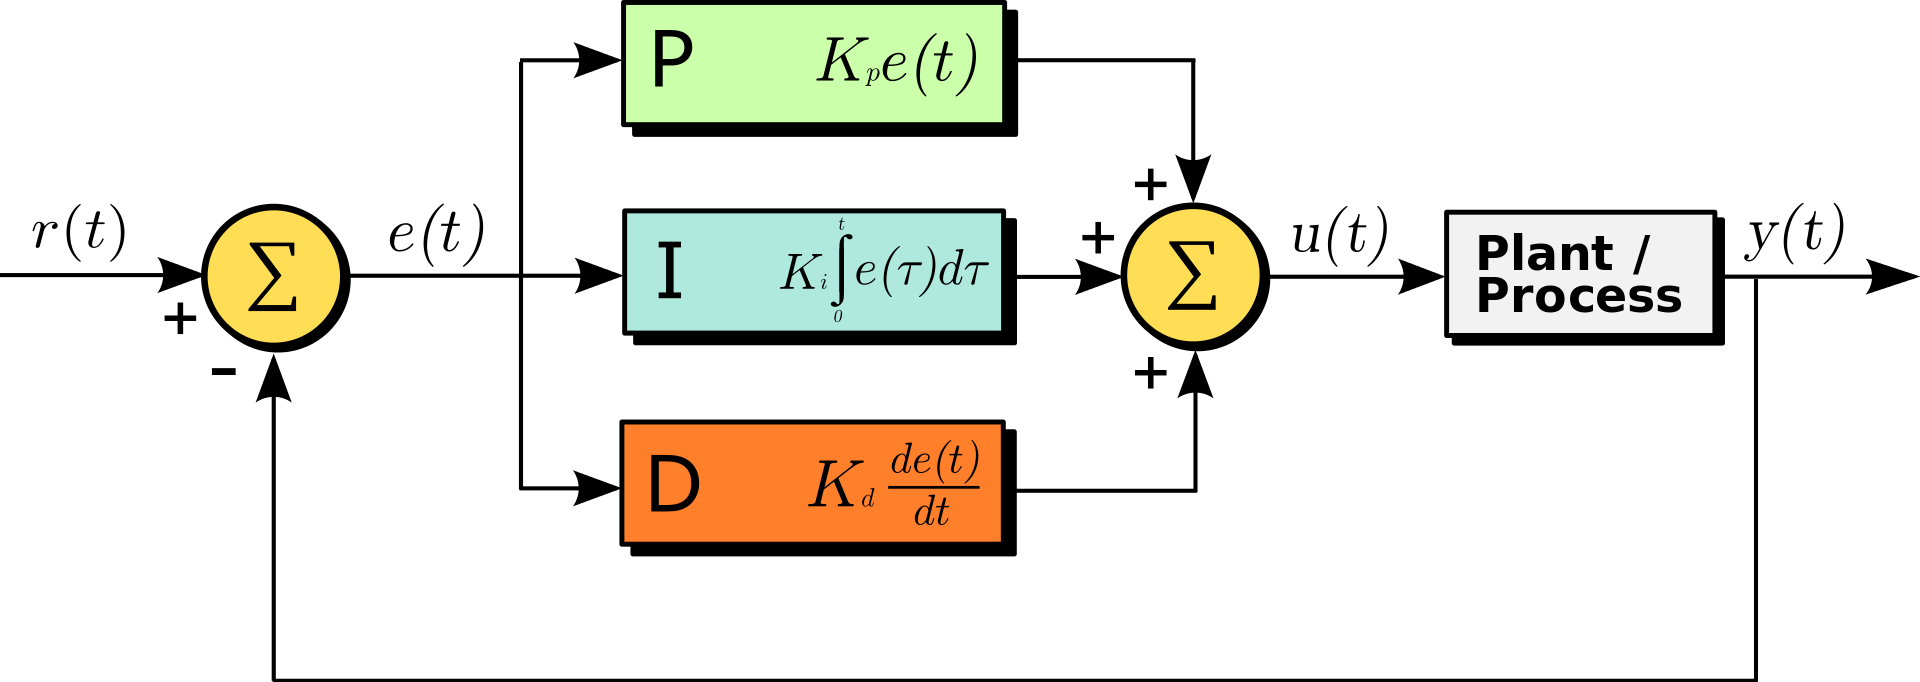
\includegraphics[width=1.0\linewidth]{pid}}
	\caption{Proportional-Integral-Derivative control driving mathematics.}
	\label{fig:pid}
\end{figure}

Fig. \ref{fig:pid} shows the driving mathematics behind the PID control system.
$r(t)$ being the current estimated state of the system derived from the various
sensors on-board. $e(t)$ is the error, which, as previously mentioned, can be
derived from a desired position and a current position. The three terms that
control the control feed sent back to the robot are weighted by parameterizable
coefficients. These coefficient are heavily system dependent and must be manually
tuned depending on physical characteristics of the robot and the control algorithm.

The three parameters, $K_p$, $K_i$, and $K_d$ each react on the error correction
of the robot in their own unique way. Here is a table of the effects each
coefficient has on the error response of the robot.

\begin{table}[htb]
	\renewcommand{\arraystretch}{1.2}
	\begin{tabularx}{\columnwidth}{|c|>{\raggedright\arraybackslash}X|>{\raggedright\arraybackslash}X|}
		\hline
		Coefficient & Too low & Too High \\
		\hline
		$K_p$ & System will not reach target state before it becomes unstable. & System will oscillate around the target state. \\
		\hline
		$K_i$ & System will undershoot the target during steady state. & System will overshoot the target during steady state. \\
		\hline
		$K_d$ & System will reach the target slowly. & System will attempt to reach the target too quickly and cause overshoot. \\
		\hline
	\end{tabularx}
	\label{tab:pid}
\end{table}

Using the guidelines outlines in table above, the PID parameters may be tuned to
allow the car to stay on the desired course. During this process, I've found it
is usually best to start with $K_i$ and $K_d$ of $0$ as the system is still able
to operate without these parameters. Adjusting three parameters all at once can
become very difficult. For the purposes of a vehicle such as this one, the integral
gain in the PID can even be left at zero for the final design. The steady state of
the car is not reachable at high speeds in turns. The derivative gain will allow the
system to adjust faster to the given desired position as it is able to take the
previous state and see how its adjustment effected the new state of the system. 

\subsection{Software Framework}

All of the subsystem of the car cause great complexity in the overall design of
the software. For this reason, each component of the software is split up into
its own independently operating subsystem. Messages can be sent synchronously
or asynchronously between components to pass data and requests between. Synchronous
message dispatch occur in the thread that the request was made, asynchronous messages
conversely will be dispatched in the thread of the component in question. This
distinction will become important in the next section when discussing the
implementation details of the system.

The component and messaging schema discussed is a very common software design for
small and medium sized robotic projects. NASA's Jet Propulsion Laboratory has
created a general purpose framework for just this purpose -- FPrime \cite{b4}.
In addition to the ability to model the generic connections and messaging between
components, FPrime also provides many tools and features that allow developers to
avoid creating boilerplate framework and hardware interaction software. This includes
features such as a commanding and sequencing paradigm in while components may define
their own commands and FPrime is able to compile a script like sequence of these
component commands \cite{b4}. \cite{b4} allows components to define their
own events (EVR - EVent Record) and telemetry (Tlm) to provide the developers and
robot operators with status logs and health statistics about the system.

\begin{figure}[htb]
	\centering
	\centerline{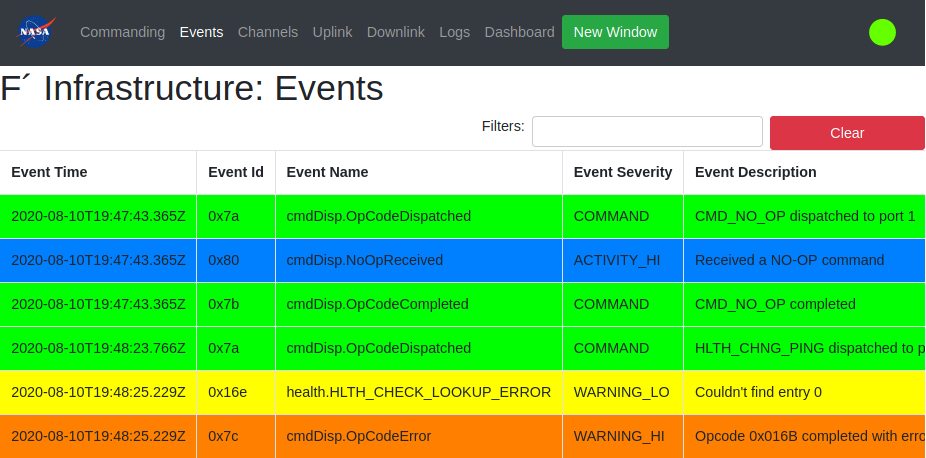
\includegraphics[width=1.0\linewidth]{gds}}
	\caption{Example of FPrime's Ground Data System showing EVRs \cite{b5}.}
	\label{fig:gds}
\end{figure}

FPrime provides an in-browser interface to view EVRs and Tlm as well as send commands
directly to the robot. The system, named the Ground Data System (GDS), receives
packets transmitted by the robot to a server hosted by the same machine running GDS.
The is the developer's main interface to the robots current status, logs, and
commanding. Fig. \ref{fig:gds} shows the EVR menu in GDS with various of the event
severity levels. This is a live feed from the robot and is transmitted to GDS with
a tunneled connection protocol (TCP) connection to the GDS server.

This software framework was selected as it was optimal to avoid extra work with
debugging and allowed most of the focus of the project to lie on the design of the
vision and navigation subsystems.

\section{Proposed Method}

This section will discuss the implementation details of the software and hardware
implementation of the car. This section will reference the code found
in a Github repository: \url{https://github.com/Kronos3/vo-cmpe460.git}. It will
be important to first discuss the layout of the code.

The component implementation files discussed in this paper will be found in `Rpi'.
Every subdirectory found here will model a separate component. This is with the
exception of `Top' that will provide the FPrime topology to initialize and interconnect
all of the components. `Top' also includes the main entry point of the software
which will perform the nominal boot-up sequence.

Components must provide define their message ports used to interface with other
components. These definitions live in the `ComponentNameComponentAi.xml' file
that is shipped with every component. Components may also optionally define
parameters, events, telemetry, and commands which can be found in their corresponding
`.xml' file. These files are inputs into FPrime's automatic programming (autocoding)
\cite{b4}. FPrime's autocoding will provide the generic boilerplate code such as
component base classes. The developer will then extend these autocoded base classes
with access to the autocoded EVRs and Tlm.

Reusable sequences used to set up the system or run certain algorithms can be
found in the `seqs' directory. These files are FPrime sequences have a very
simple syntax:

\begin{verbatim}
R00:00:10 component.COMMAND ARG1 ARG2
\end{verbatim}

This command will wait 10 seconds and then dispatch `COMMAND' to `component'.
FPrime scripting is used to build the vision pipeline as well as set up a video
live stream and begin the navigation algorithm.

\subsection{Hardware}

The car operates with two compute boards. As previously mentioned,
an MSP432P401R microcontroller is used to provide the PWM signals the motors.
There are two throttle motors on the rear wheels and a single servo that will
control the servo arms. 

\begin{figure}[htb]
	\centering
	\centerline{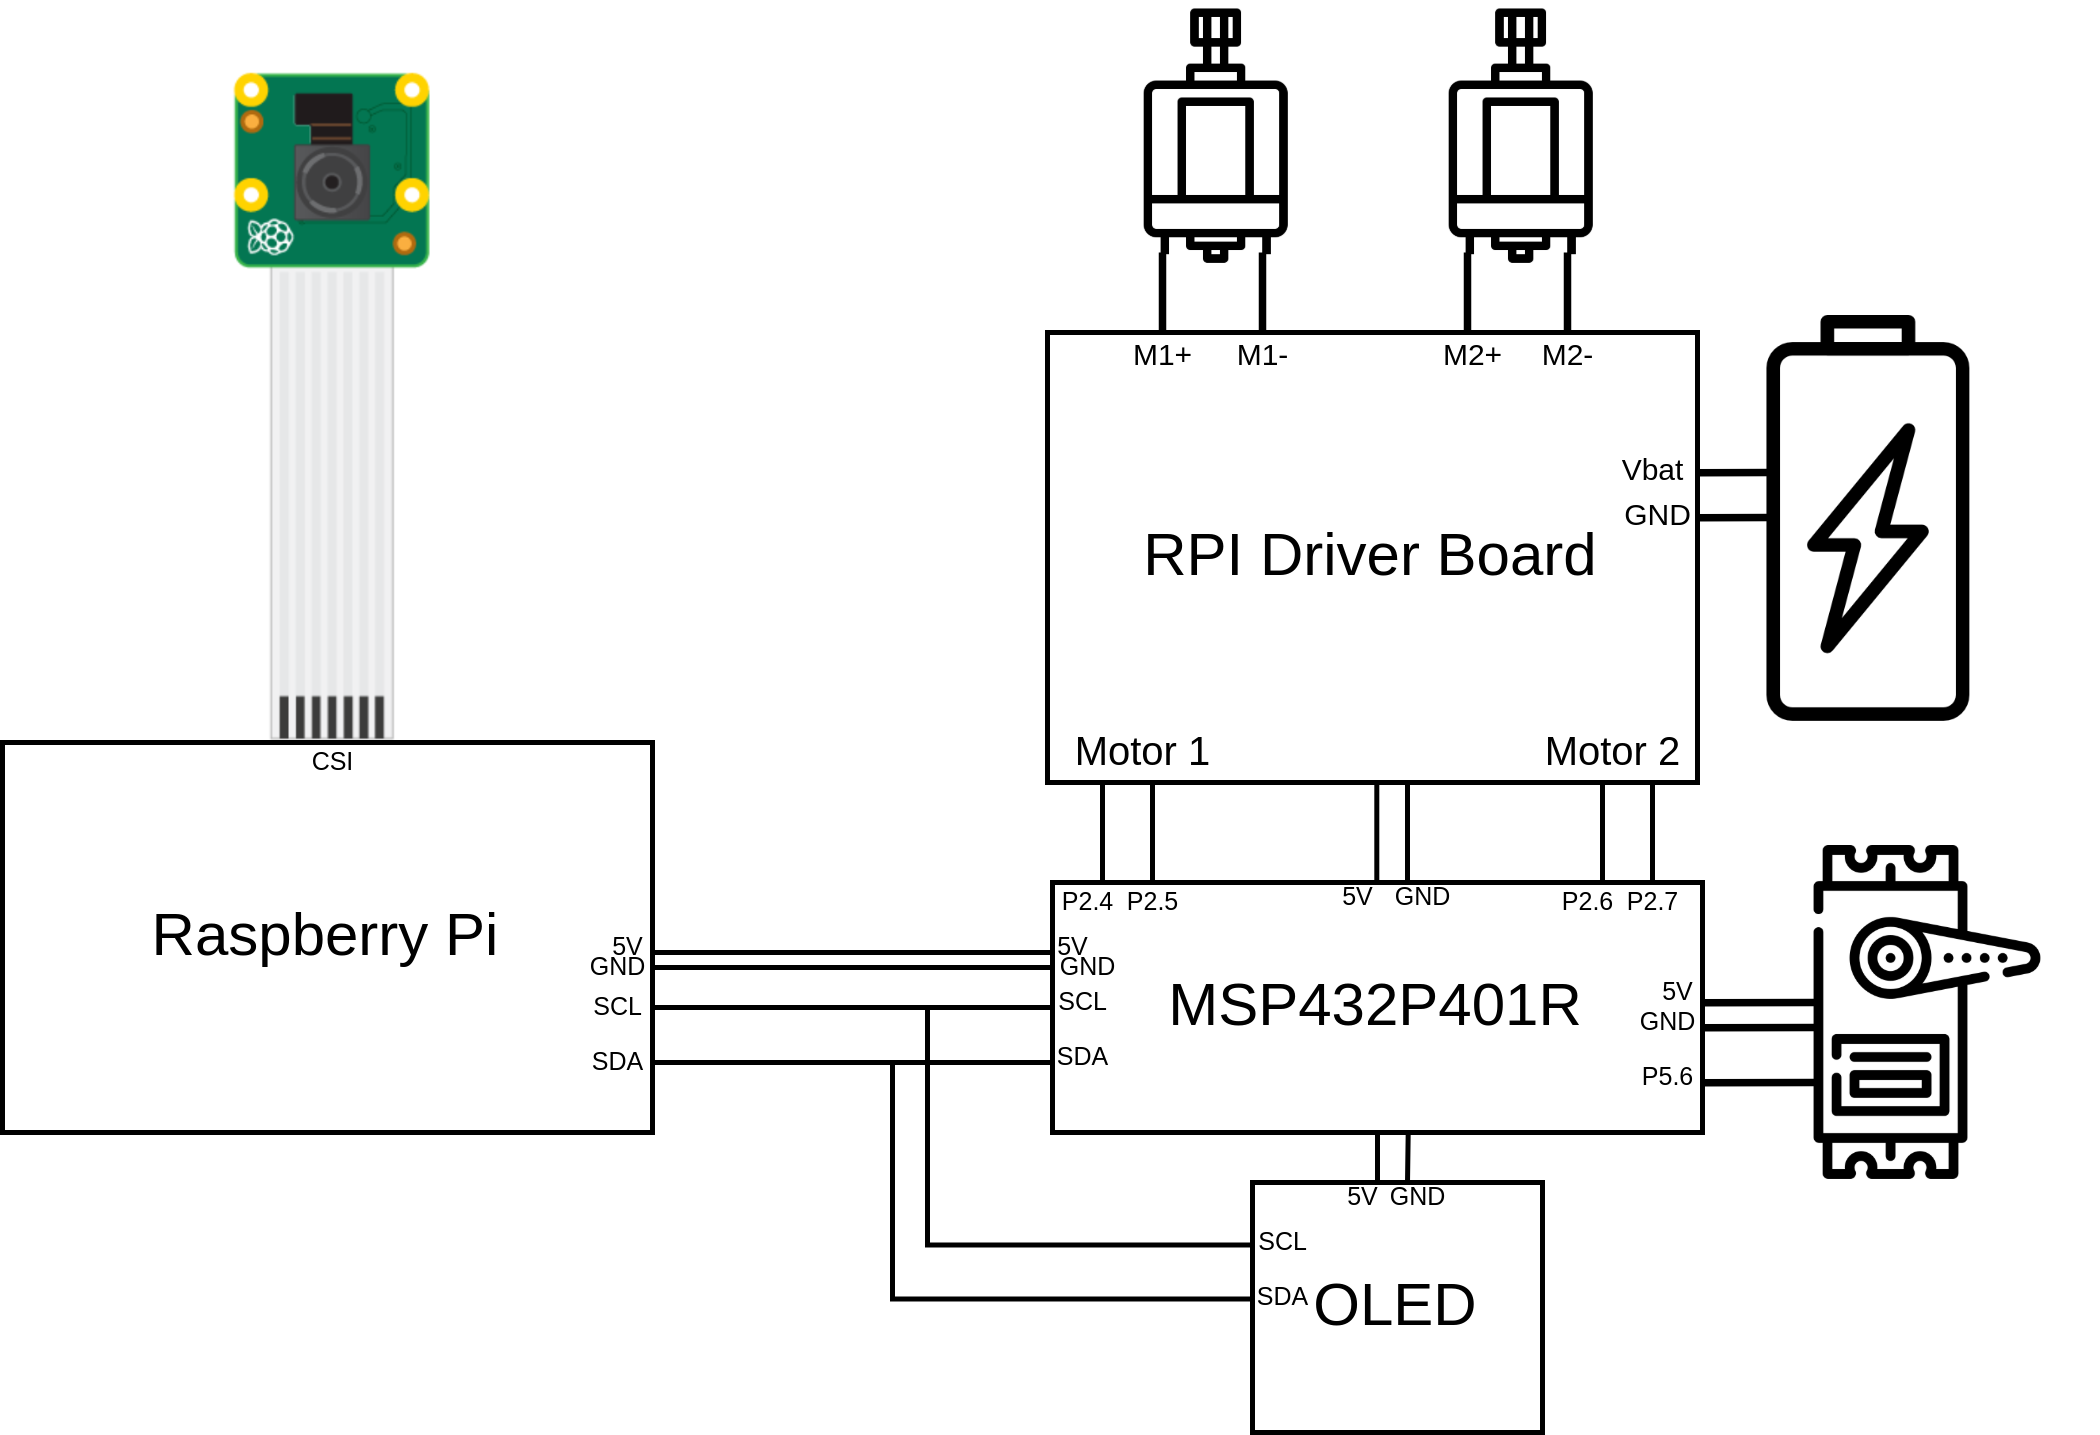
\includegraphics[width=1.0\linewidth]{wiring}}
	\caption{Hardware wiring of Raspberry Pi, MSP432P401R and other hardware.}
	\label{fig:hardware}
\end{figure}

Fig. \ref{fig:hardware} shows the basic wiring scheme of the car. An
Inter-Integrated Circuit (I2C) connection is used to send commands from the 
Raspberry Pi to the MSP432P401R. An organic light-emitting diode (OLED) display
is also connected to the common I2C bus. The display is used to print the
internet protocol (IP) address of the Raspberry Pi on boot-up so that a user will
where to shell into via a secure-shell (SSH) connection. The Raspberry Pi
is the master device in the I2C chain. The Pi is able to arbitrate the common I2C
bus by providing the device's unique address before each packet. This will allow
the Pi to command both the OLED display and MSP432P401R via the same I2C interface.

The Raspberry Pi Camera Module shown in the upper left corner of Fig.
\ref{fig:hardware}, is connected via a ribbon cable to the Pi's
Camera Serial Interface (CSI). Due to field-of-view (FOV) limitations of the
default camera module's lens, a Fisheye lens with $180^{\circ}$ FOV is used.

\begin{figure}[htb]
	\centering
	\centerline{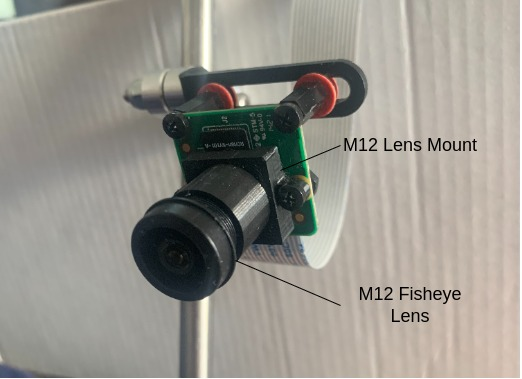
\includegraphics[width=0.7\linewidth]{camera_annotated}}
	\caption{Camera lens and mount.}
	\label{fig:camera}
\end{figure}

Fig. \ref{fig:camera} shows the physical configuration of the fisheye lens
with the camera module. The M12 lens mount shown in Fig. \ref{fig:camera} is a
3D printed lens mount meant for the M12 thread present on the lens in use.
Although this lens will cause considerable distortion, it is vital to use a
high horizontal FOV lens to be able to see both edges of the track immediately
next to the car. The default lens on the camera module has a horizontal
FOV of $53^{\circ}$ \cite{b6}. A small horizontal FOV such as this one would mean
the car would see the track too far ahead of itself.

\subsection{Component Topology}

This section will discuss the general layout and interaction between all the system
components. Also the vital components are discussed though there are many other
supporting builtin FPrime components that are not shown. Connections between components
indicate some relationship and flow of data.

\begin{figure}[htb]
	\centering
	\centerline{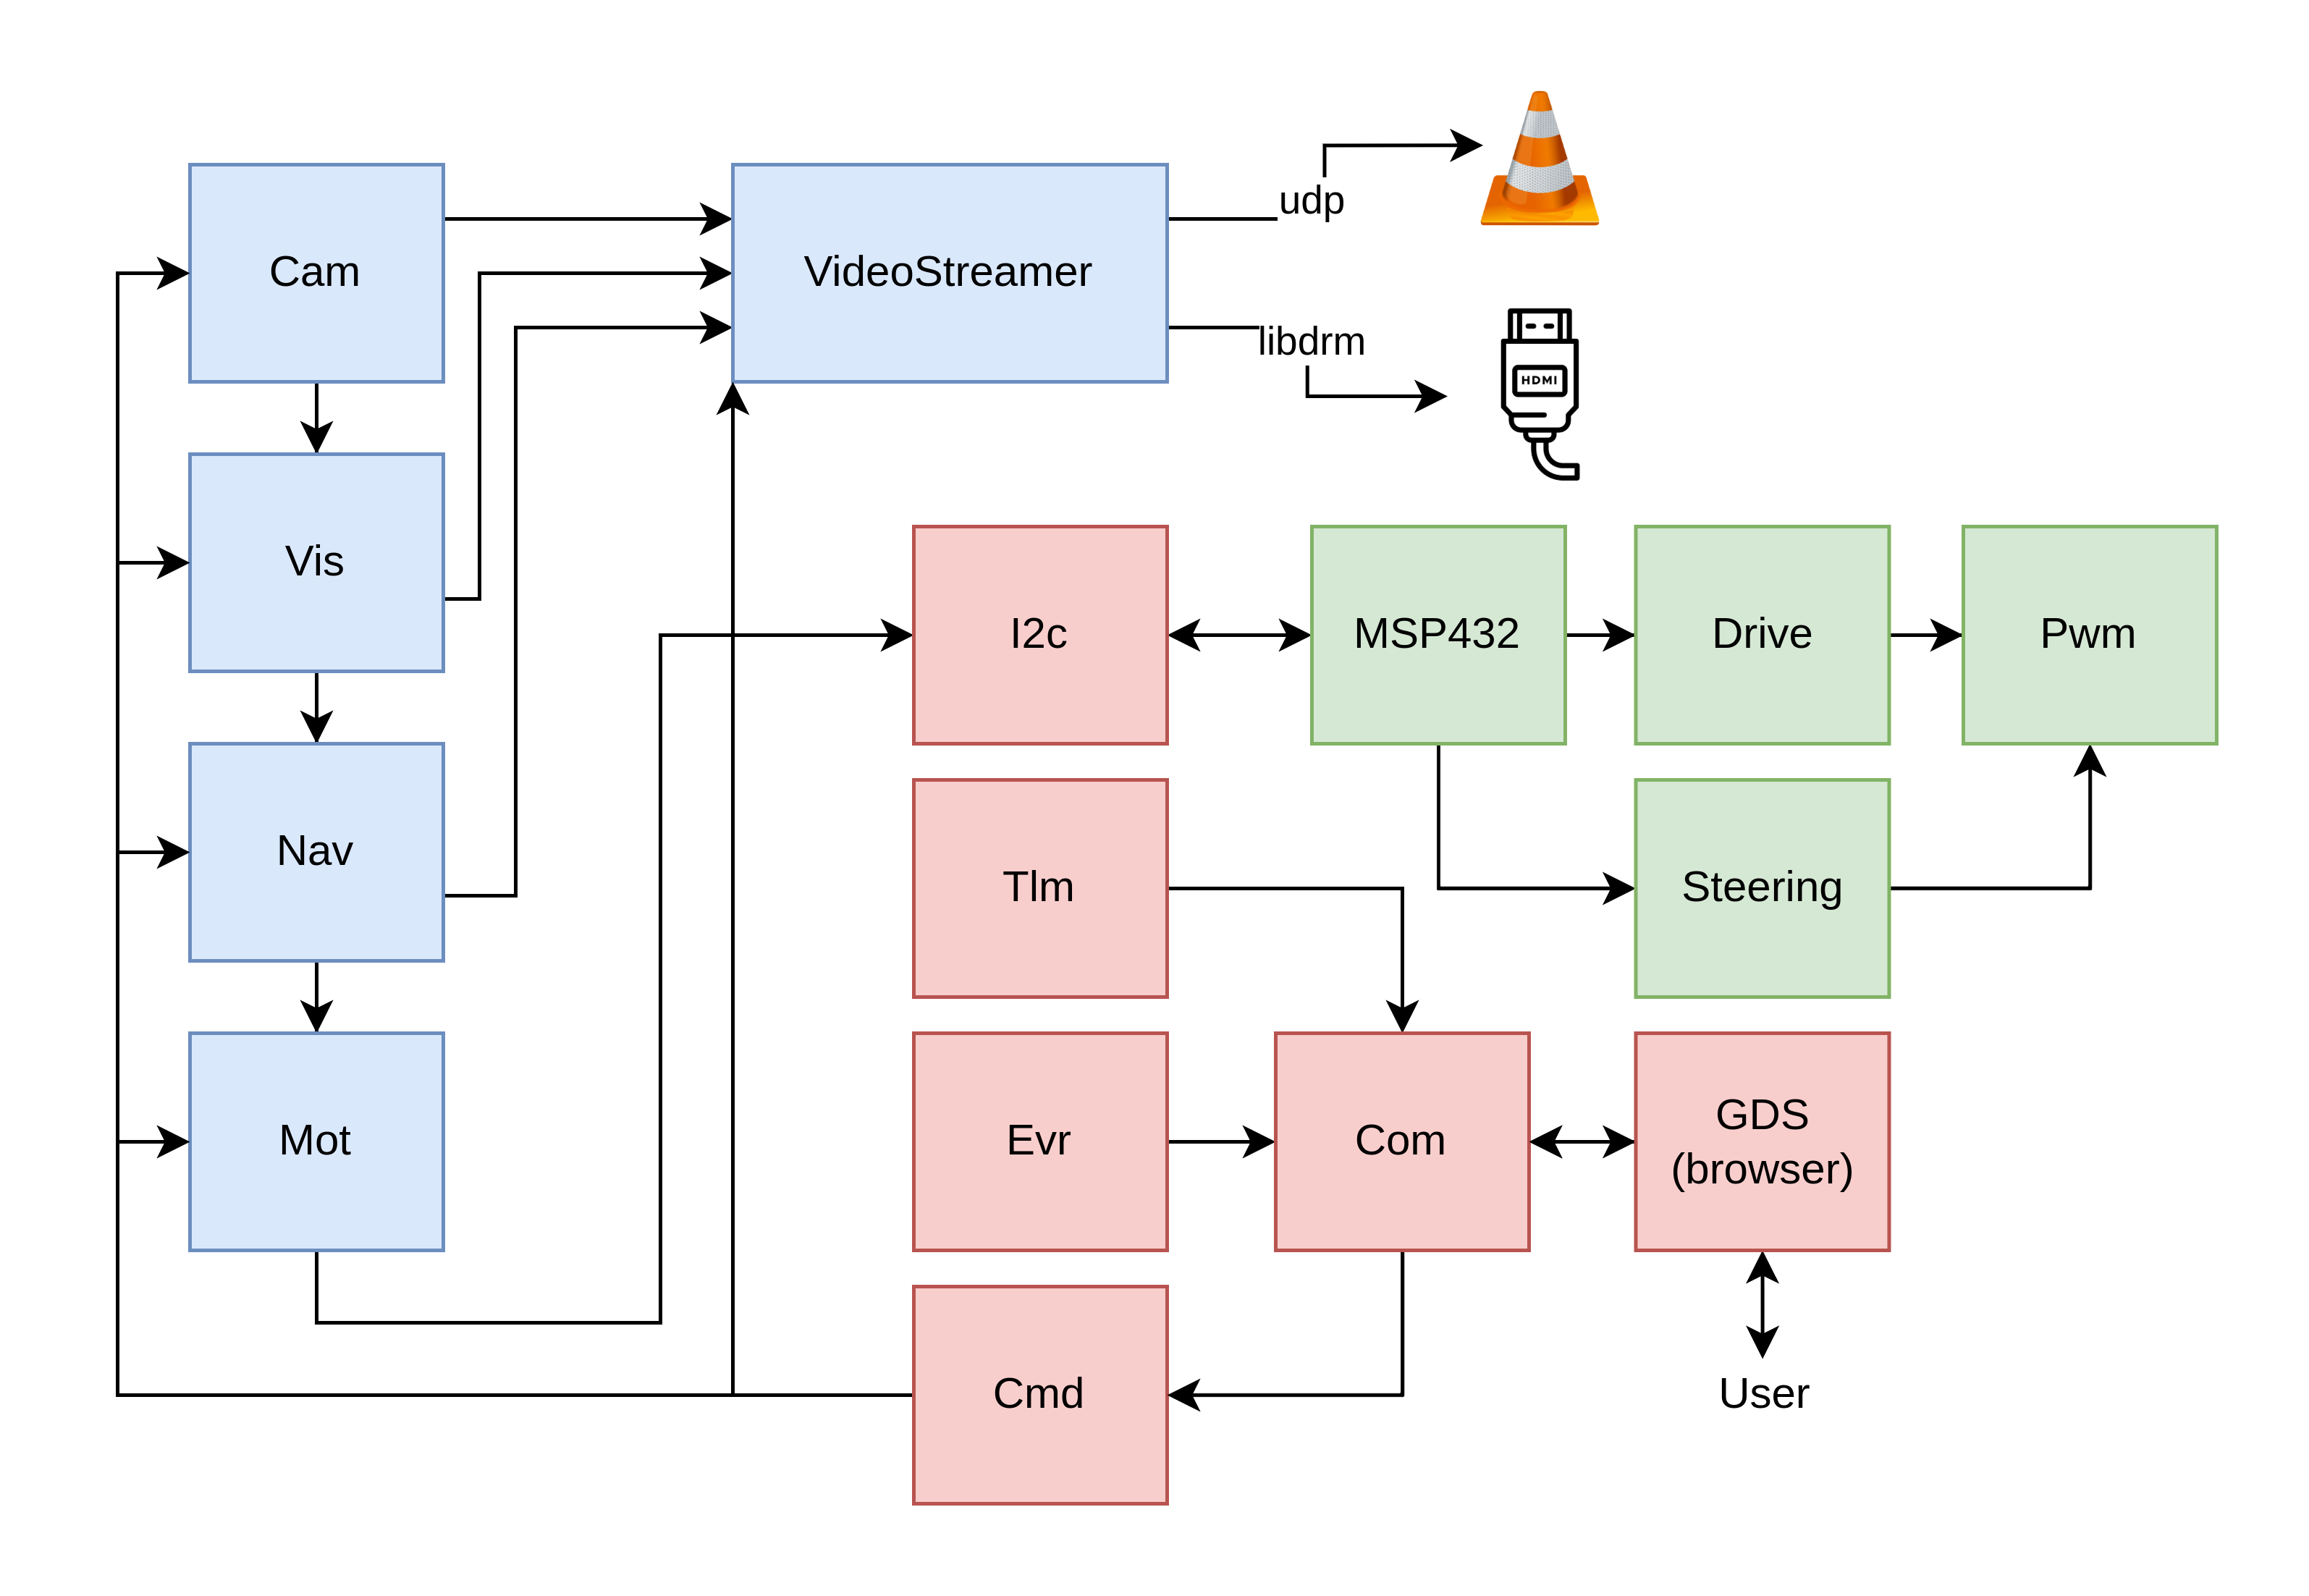
\includegraphics[width=1.0\linewidth]{block}}
	\caption{Full system component topology.}
	\label{fig:block}
\end{figure}

Fig. \ref{fig:block} shows the basic component layout of the project. The camera
will acquire image frames and is able to stream to the VideoStreamer or the
vision component (Vis). Similarly, Vis is able to stream to the VideoStreamer or
to the navigation component (Nav). The video streamer is a component that is able to
draw image frames on an HDMI display or to encode a sequence of frames as an H.264
video live stream. This live stream can be viewed externally by a VLC media player
client. The VideoStreamer is imperative to development and debugging as image frames
may be annotated to show algorithms in action.

The MSP432P401R microcontroller is connected to the I2C bus and, as discussed before,
will provide the motor control for the DC and servo motor. Both the steering and
the dc modules are small wrappers around the pwm module. The pwm module will interface
with the TimerA peripheral on-board the MSP432P401R to generate hardware triggered
PWM waves.

\subsection{Motor (Mot)}

The microcontroller's sole purpose in this design is to control the motors. The
Raspberry Pi needs a communication protocol for encoding a command to the
microcontroller. The `Mot' component will handle this interaction by
encoding a command packet and sending it out over the I2C bus. A command packet
will consist of two single byte fields: opcode and value.

The value field is interpreted differently per command opcode. Because field the
value is only a single byte, valid values range from 0 to 255. Opcodes can be found
in `Mot/Types/MSP432PwmOpcodeEnumAi.xml'. The DC motors can be controlled with
the FORWARD or BACKWARD packet opcodes on each motor. A value of 0 will stop the
motor in question while a value of 255 will run the motor at maximum speed in the
direction noted by the opcode. The SERVO opcode will provide steering control. A
value of 0 will turn the servo completely left, while 255 will turn it completely
right.

Mot will allow control from other components via a more generic synchronous
messaging port. The steering port will allow floating point values from $-1$ (left)
to $1$ (right), while the throttle port will allow two throttle values from $-1$
(backwards) to $1$ forwards for each of the two DC motors. Mot is therefore responsible
for encoding a software friendly floating point number, to a hardware friendly command
packet to send to the microcontroller.

\subsection{Camera (Cam)}

The camera component (Cam) is responsible for interfacing with the camera. This
software will use libcamera to interface directly with the kernel driver and the
hardware. Once a camera stream is initialized, Cam will need to manage the camera
buffers sent and received from the camera. Cam needs to make an acquisition request
to libcamera by passing it a frame buffer. Multiple frame buffers may be requested
at once. The camera is configured to acquire images at 30 FPS. When an image is
acquired the camera will send a filled image buffer back to Cam.

Looking at Fig. \ref{fig:block}, Cam, Vis, Nav, and VideoStreamer are all
interconnected. These connections refer to image frames being passed through out
the components. It is the responsibility of each component to either pass the
image frame to another component, or to return the image frame to the camera. When
the frame is returned to the camera, it is reused for acquisition.

For use with the car, the camera will capture 1640x1232 pixel image frames at 30 FPS. The camera's saturation is zeroed as a gray-scale image is used for image processing. The white balance is set to auto which will help calibrate the color balance in different room environments. All other camera settings can be found in the `cam\_configure' sequence.

\subsection{VideoStreamer}

VideoStreamer is a very simple component that is able to display image frames on select-able mediums. The VideoStreamer supports displaying to a High-Definition Multimedia Interface (HDMI) connected directly to the Pi or to stream over the network to a VideoLAN Client (VLC) using a UDP connection. The HDMI display is able to draw memory-mapped Direct Memory Access (DMA) memory regions which are specially allocated by the Linux kernel. These memory mapped regions can be written to and read from directly by the integrated graphics processing unit (GPU). Camera frame buffers also must reside in these memory mapped regions as the Raspberry Pi camera will apply hardware accelerated post-processing before releasing the image to the camera client. This means that the original image buffer provided by the camera process must be passed directly to the HDMI streaming process and the buffer must be held until another frame is ready to display. This logic because quite complex in terms of managing the life cycle of each frame buffer. When a frame buffer is no longer in use, it must return to the camera to acquire a new frame. To keep track of when a frame buffer is in use, a reference counter is used to keep track of the lifetime of the buffer. This idea is the Python programming language uses to keep track the life cycle of its objects \cite{c7}.

Because HDMI is only useful in the early stages of development, a separate display method is used to transmit encoded video over the network. Transmitting each individual raw frame over the network would be extremely inefficient and provide for poor results. Instead, the video is encoded into an H.264 video stream and transmitted over the network via a UDP connection. The VideoStreamer will leverage the Raspberry Pi's hardware H.264 video encoder via the videodev2 library to provide accelerated encoding capabilities. Although in noisy environments the UDP stream may occasionally be interrupted briefly, the H.264 encoder and UDP connections are able to keep up with the framerate requirements presented by this project.

\subsection{Vision (Vis)}

The Vis component is possibly the most important component in the robot. The purpose
of this component is to process the image frame in such a way that the navigation
component can use it for controlling the car. Vision will receive raw image frames
from the camera and apply a series of transformations to the image. Each transformation
is known as a pipeline stage where the culmination of all the stages is known as the
pipeline.

The entire pipeline in Vis is completely modular. This means that the pipeline stages
can be added to the pipeline via a simple command. Pipeline stages may have parameters
associated with them which can similarly be set via command. This modular design allows
for easy changes to be made to the vision pipeline as well as allowing multi-purpose
use of the vision component. For example, a race vision pipeline can be initialized
during the race boot-up sequence to perform edge detection. Similarly, a calibration
pipeline can be set up to compute the camera pose and be used for perspective correction. Another advantage of this method is simplicity in implementation. Each pipeline stage is an extremely simple processing step and therefore reduces the chance of introducing errors.

\subsubsection{Edge Detection}

When designing the race pipeline, the input into the navigation must be considered. The purpose in the Vis component is to apply transformation to the image that will provide Nav with information to place itself on the track. For this project, the most important features to extract from the image frame are the edges of the track. We would therefore expect Vis to transform the raw image to only include track lines. This can be done with an edge detector.

\begin{figure}[htb]
\begin{minipage}[b]{.48\linewidth}
	\centering
	\centerline{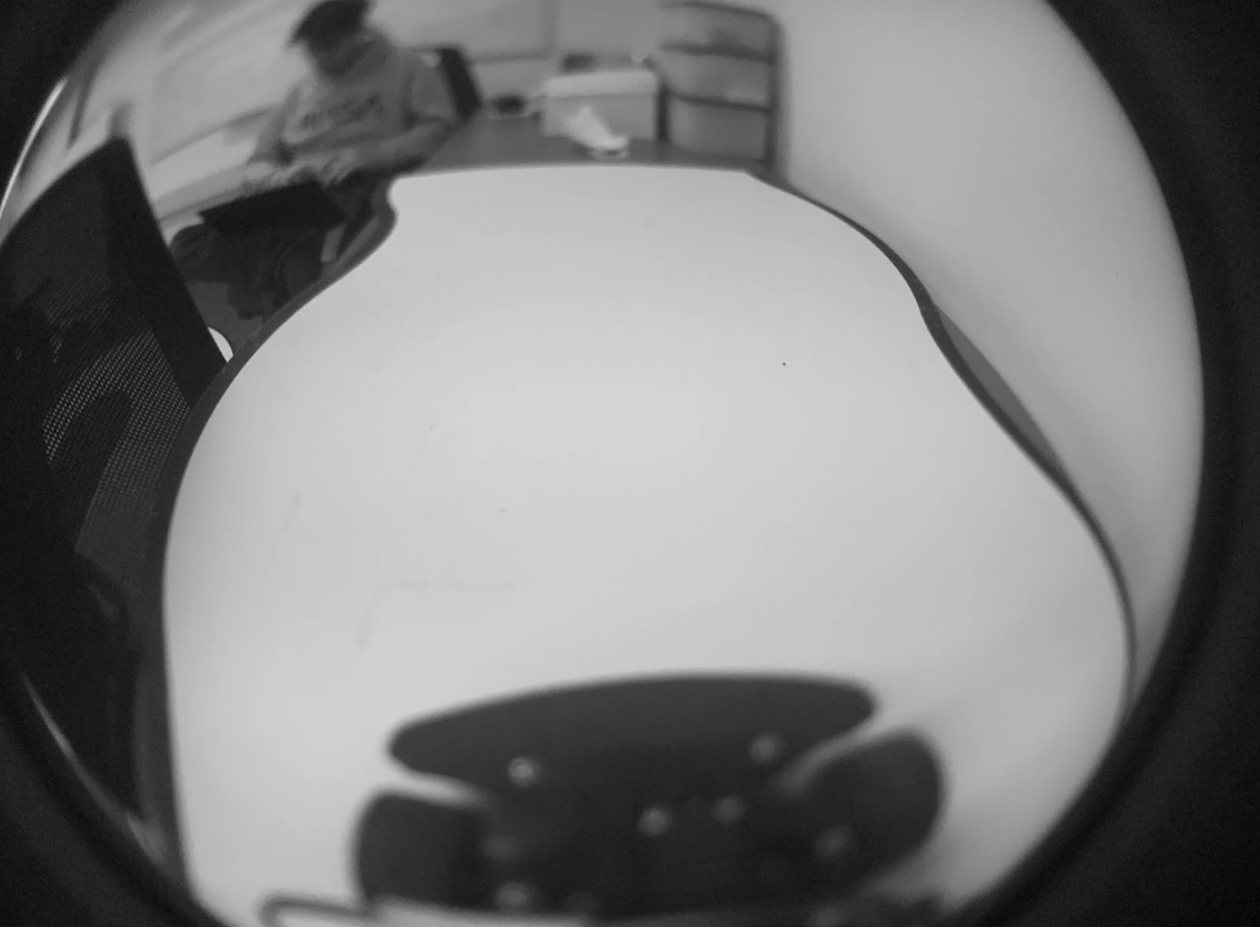
\includegraphics[width=4.0cm]{vis_figs/raw}}
	%  \vspace{1.5cm}
	\centerline{(a) Raw image}\medskip
\end{minipage}
\hfill
\begin{minipage}[b]{0.48\linewidth}
	\centering
	\centerline{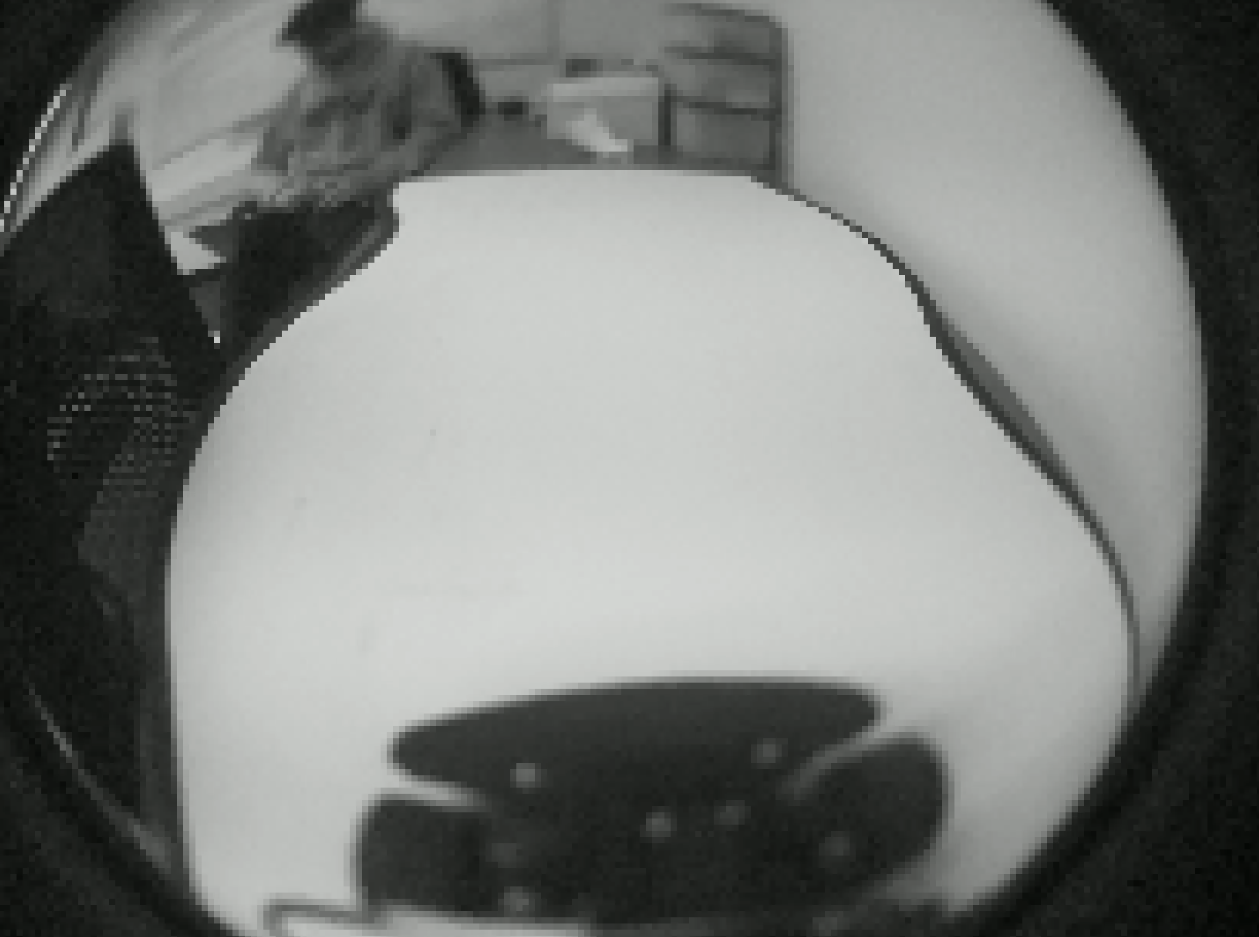
\includegraphics[width=4.0cm]{vis_figs/downscale}}
	%  \vspace{1.5cm}
	\centerline{(b) Downscale (x16)}\medskip
\end{minipage}
%
\begin{minipage}[b]{.48\linewidth}
	\centering
	\centerline{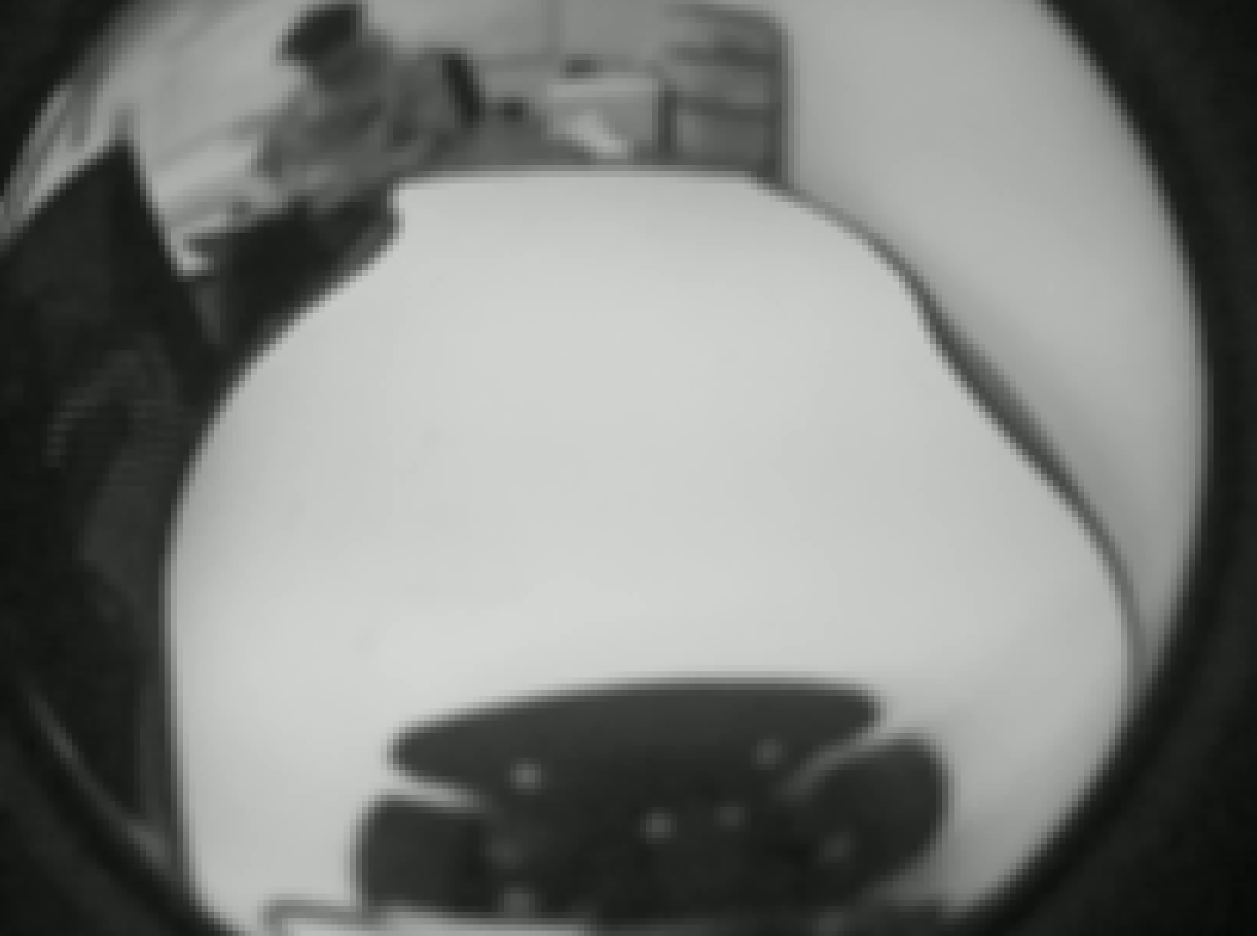
\includegraphics[width=4.0cm]{vis_figs/gaussian}}
	%  \vspace{1.5cm}
	\centerline{(c) Gaussian blur}\medskip
\end{minipage}
\hfill
\begin{minipage}[b]{0.48\linewidth}
	\centering
	\centerline{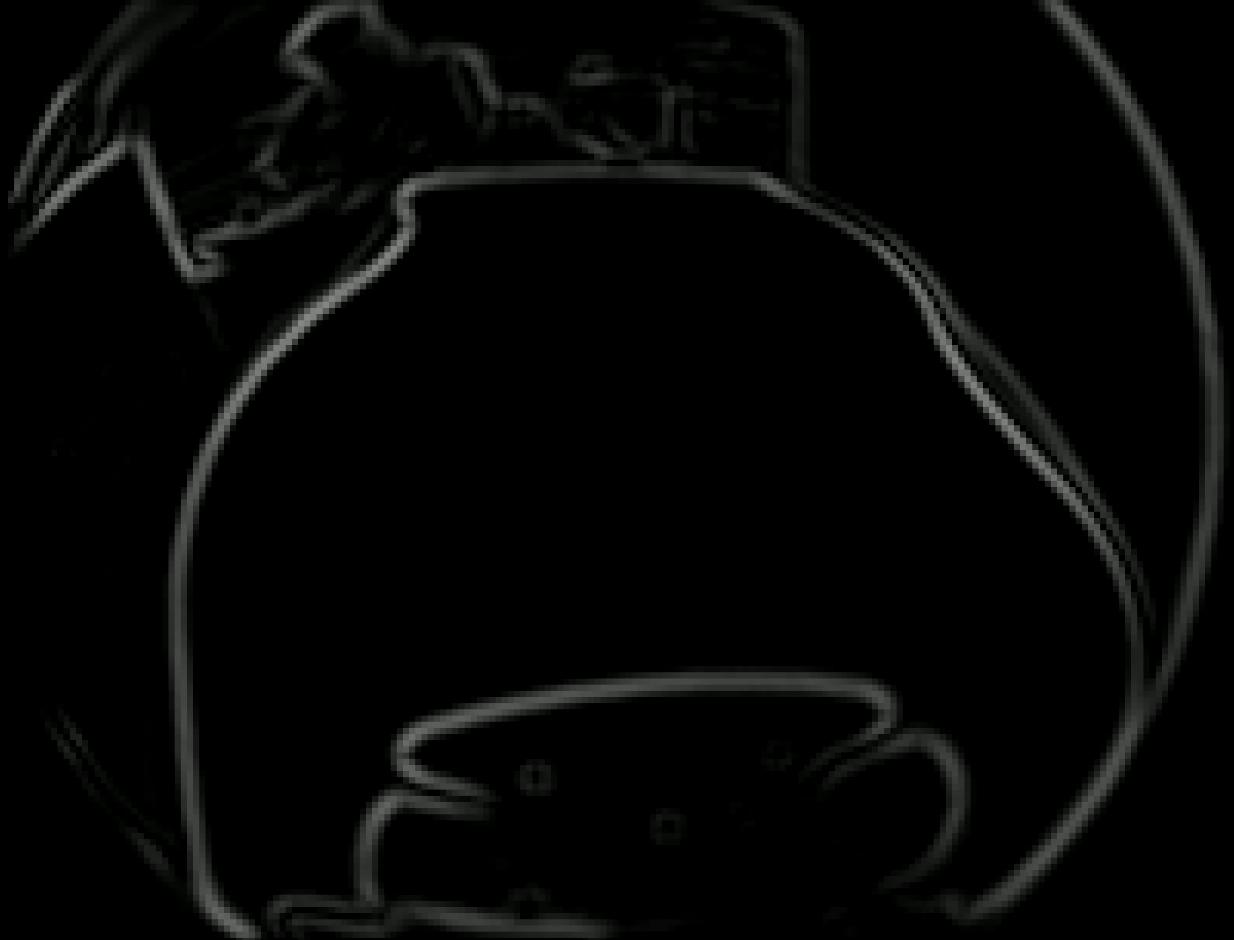
\includegraphics[width=4.0cm]{vis_figs/gradient}}
	%  \vspace{1.5cm}
	\centerline{(d) Sobel XY edge filter}\medskip
\end{minipage}
%
\caption{First four stages of the race pipeline applied to the
	same image.}
\label{fig:vis1}
%
\end{figure}

Fig. \ref{fig:vis1} shows the an image of the car on a section of the track. This test is especially interesting because the track is next to a white wall. With a 16x downscale (Fig. \ref{fig:vis1} (a))applied to the image to achieve reasonable performance on the Raspberry Pi, it is difficult even to the human eye to make out the edges of the track. The Sobel filter however if able to appropriately find these edges using its convolution kernel. The purpose in applying a Gaussian blur filter to the image before the Sobel filter is to essentially apply a low pass digital filter. This will smooth out noisy regions as well as make sure track edges are seen thicker and more solid. Like the Sobel filter, the Gaussian blur is a convolution kernel however, instead of applying a gradient functor, a weighted average of surrounding pixels is used. This racing pipeline will use a 3x3 kernel as it has reasonable computational performance and yield an acceptable output.

\subsubsection{Pose Calibration}

When working with camera's on robots, it is very common to calibrate the pose of the camera \cite{b1} \cite{b3}. This refers to computing the rotation and translation relative to a known point on the ground plane. Calibrating the pose would allow the image frame to be transformed into "birds-eye" view orientation. This orientation is obviously advantageous to the navigation algorithm as its easier to form a navigational path when looking directly above.

OpenCV supports pose calibration via its calib3d library. This project uses a chessboard calibration target as it is the most commonly used target for pose calibration. This is simply a set of black squares on white paper. OpenCV is able to find the corners between the squares and provide the end user with a set of image coordinates. Because these corners are at known positions on the ground plane, OpenCV is able to derive pose information from the location of the these squares.

\begin{figure}[htb]
	\centering
	\centerline{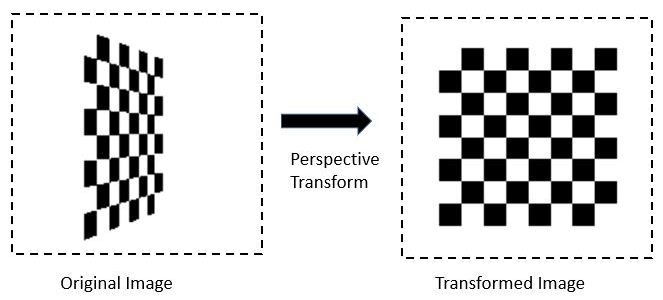
\includegraphics[width=1.0\linewidth]{perspective}}
	\caption{Perspective transform applied to chessboard image.}
	\label{fig:perspective}
\end{figure}

Fig. \ref{fig:perspective} shows an example of a chessboard with a perspective transform applied to it. To build the transformation matrix, two sets of four
points must be provided. The first set of four points will correspond to the outer corners of the chessboard calibration target on the raw image frame. The next four points will correspond to the outer corners on the perspective transformed image frame. Vis will apply a perspective transform on the filtered image frames shown in Fig. \ref{fig:vis1}.

\begin{figure}[htb]
	\begin{minipage}[b]{.48\linewidth}
		\centering
		\centerline{\includegraphics[width=4.0cm]{vis_figs/vis\_intersection}}
	\end{minipage}
	\hfill
	\begin{minipage}[b]{0.48\linewidth}
		\centering
		\centerline{\includegraphics[width=4.0cm]{vis_figs/vis\_straight}}
	\end{minipage}
	\caption{Vis processed images of intersection and straightaway.}
	\label{fig:vis2}
\end{figure}

The full vision pipeline's results shown in Fig. \ref{fig:vis2} show a combination of processing done in Fig. \ref{fig:vis1}, a warp transform, and finally a binary threshold to create hard edges. Fig. \ref{fig:vis2} shows very good results near the center of the image with relatively straight lines on the straightaway (right). 

\subsection{Navigation (Nav)}

\section{Results}
\section{Conclusion}

\begin{thebibliography}{00}
\bibitem{b1} J. N. Maki, D. Gruel, C. McKinney, M. A. Ravine, M. Morales, D. Lee, R. Willson, D. Copley-Woods, M. Valvo, T. Goodsall, J. McGuire, R. G. Sellar, J. A. Schaffner, M. A. Caplinger, J. M. Shamah, A. E. Johnson, H. Ansari, K. Singh, T. Litwin, R. Deen, A. Culver, N. Ruoff, D. Petrizzo, D. Kessler, C. Basset, T. Estlin, F. Alibay, A. Nelessen, and S. Algermissen, “The Mars 2020 engineering cameras and microphone on the Perseverance Rover: A next-generation imaging system for mars exploration - space science reviews,” SpringerLink, 24-Nov-2020. [Online]. Available: https://link.springer.com/article/10.1007/s11214-020-00765-9. [Accessed: 20-Apr-2022]. 
\bibitem{b2} “Power consumption benchmarks,” Power Consumption Benchmarks | Raspberry Pi Dramble. [Online]. Available: https://www.pidramble.com/wiki/benchmarks/power-consumption. [Accessed: 18-Apr-2022].
\bibitem{b3} A. Rosebrock, “Raspberry Pi For Computer Vision,” PyImageSearch, 08-May-2021. [Online]. Available: https://pyimagesearch.com/2019/04/05/table-of-contents-raspberry-pi-for-computer-vision/. [Accessed: 18-Apr-2022].
\bibitem{b4} R. L. Bacchino, T. K. Canham, G. J. Watney, L. J. Reder, and J. W. Levison, “F Prime: An Open-Source Framework for Small-Scale Flight Software Systems,” NASA JPL Beacon, 04-Aug-2018. [Online]. Available: https://trs.jpl.nasa.gov/handle/2014/48425. [Accessed: 20-Apr-2022]. 
\bibitem{b5} “A brief guide to the F´ ground data system,” F´. [Online]. Available: https://nasa.github.io/fprime/UsersGuide/gds/gds-introduction.html. [Accessed: 20-Apr-2022].
\bibitem{b6} “Raspberry pi documentation,” Camera. [Online]. Available: https://www.raspberrypi.com/documentation/accessories/camera.html. [Accessed: 20-Apr-2022].
\bibitem{c7} “Reference counting,” Reference Counting - Python 3.10.4 documentation. [Online]. Available: https://docs.python.org/3/c-api/refcounting.html. [Accessed: 23-Apr-2022]. 
\end{thebibliography}

\end{document}